\documentclass[hyperref,UTF8]{ctexart}    
	\usepackage{amsmath}
	\usepackage{amssymb}	
	\usepackage[a4paper,bindingoffset=0.2in,%
            left=1in,right=1in,top=1in,bottom=1in,%
            footskip=.25in]{geometry}
\usepackage{graphicx}
\usepackage{enumerate}
\usepackage{url}
\usepackage{hyperref}
\usepackage{pbox}
\usepackage{CJKutf8}


\begin{document}
\title{报告}
\author{盛嘉成, 14307130038 \\ 计算机科学与技术学院}
\maketitle
\section{Regreesion \& KNN}
\subsection{Logistic Regression}
logistic回归的模型首先把x属于类$C_1$后验概率写成logistic sigmoid函数的形式:
\[p(C_1|x)=\frac{p(x|C_1)p(C_1)}{p(x|C_1)p(C_1)+p(x|C_2)p(C_2)}=\frac{1}{1+e^{-a}}\]
\par 其中
\[a=\ln{\frac{p(x|C_1)p(C_1)}{p(x|C_2)p(C_2)}}\]
\par 然后核心的,我们假设a可以由x的线性函数拟合$p(C_1|\phi)=\sigma(\omega^{T}\phi)$,于是我们就可以使用最大似然方法估计参数$\omega$。对于N个训练样本,M+1维基函数(人为添加一个值为1的基,以方便设置偏置参数$\omega_0$),带上L2正则化项后,相应的误差函数为:
\[E(\omega)=-\sum_{n=1}^{N}(t_n\ln{y_n}+(1-t_n)\ln{(1-y_n)})+\frac{\lambda}{2} \sum_{j=1}^{M}{\omega_j}^2\]
\par $t_n$为样本的标签(真实类别),$y_n=\sigma(\omega^{T}\phi)$
\par 最小化误差函数的方法有多种,自己实现了两种,第一种是直接采用梯度下降的方法:
\[\omega_{new} =\omega_{old}-\eta \frac{\partial E(\omega)}{\partial \omega} \]
\par 由于正则化项不包含偏置参数,所以独立开$\omega_0$,有:
\[\frac{\partial E(\omega)}{\partial \omega_0}=\sum_{n=1}^{N}(y_n-t_n)\phi_{n0}\]
\[\frac{\partial E(\omega)}{\partial \omega_j}=\sum_{n=1}^{N}(y_n-t_n)\phi_{nj}+\lambda \omega_j\]
\par 写成矩阵形式:
\[\omega_{new} =\omega_{old}-({\Phi}^{T}(y-t)+\lambda [0,\omega_1,\omega_2,...,\omega_M]^T)\]
\par 其中$\Phi$为所有样本基函数,在我们的实验中,除了第一列为人为添加的1,后57列是邮件的57个特征,每行对应一个训练样本。

\par 另一种方法是利用Newton法逼近梯度为0的位置:
\[\omega_{new} =\omega_{old}-H^{-1}\nabla E(\omega)\]
\par 其中H为E关于$\omega$的二阶导构成的Hessian矩阵:
\[H={\Phi}^{T}(R)\Phi+\lambda I^{*}\]
\par $R$是由$y_j(1-y_j)$在对角线上组成的对角阵,$I^{*}$除了第一行第一列的元素为0,其他位置和M+1阶单位阵相同。
\par 以上即logistic回归的模型和参数估计方法。接下来的实验结果部分除了问题v两种方法的对比,其他问题中的实验都是用Newton法实现的。
\paragraph{(i)} 
\par 不同正则化参数下的错误率\\
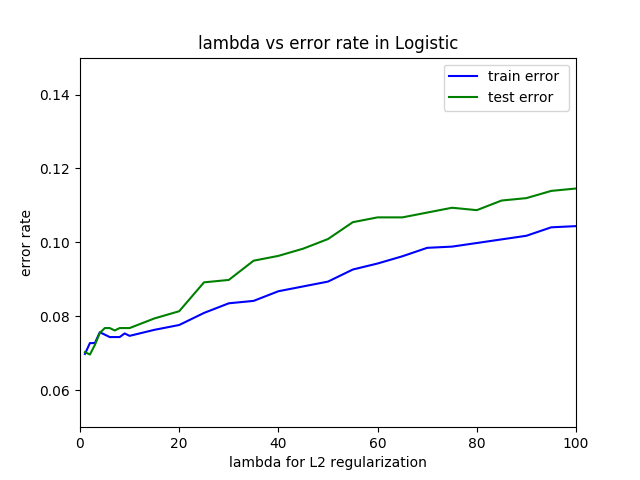
\includegraphics[height=3.8in]{Logistic-lam.png}\\
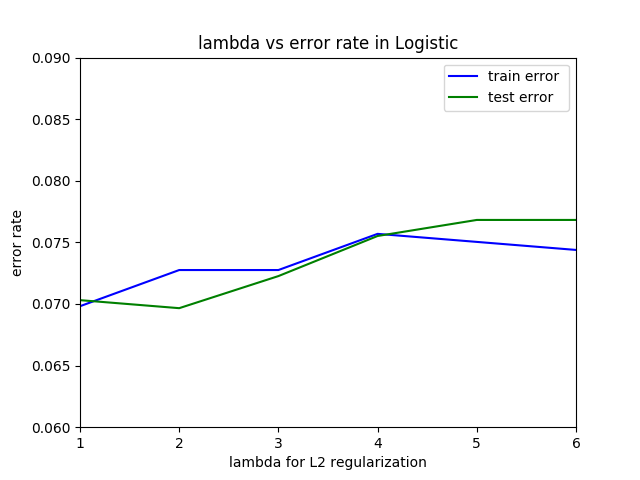
\includegraphics[width=3in]{2Logistic-lam.png}
\paragraph{(ii)}从图上可以看出,整体上随着$\lambda$增大,训练集和测试集上的错误率都逐渐增大,这是因为正则化项是为了限制参数$\omega$不太大,从而防止过拟合的现象,但是当正则化项在误差函数中的比重过大,拟合就过于泛化,出现欠拟合。
\par 从小图展现出的细节上看,对于本次实验的数据而言,当$\lambda=2$时,正则化项已足够抑制过拟合,此时估计的参数在测试集上
有最低的错误率,效果最好。
\paragraph{(iii)}框架代码中给出的几种预处理对数据分布本身的转变在上次作业已经阐述过,不再详述。从结果来看,取对数结合logistic回归对本次实验的数据有较好的分类成功率。

\begin{table}[!htbp]
% \resizebox{1.4\linewidth}{!}
  \centering
  \scalebox{1}{
\begin{tabular}{ l | c | c | c }
  \hline      
  train-err|test-err & $\lambda=1$ & $\lambda=10$ & $\lambda=100$  \\ \hline
  None  & 6.9|7.0 & 7.4|7.6 &10.4|11.4   \\ \hline
  Binarized  & 6.3|7.2 & 6.4|7.5 &9.2|9.4   \\ \hline 
  Z-normalized  & 7.4|8.7 & 7.8|8.5 &8.9|9.5   \\ \hline
  Log  & 5.0|5.9 & 5.1|5.9 &6.3|6.9   \\ \hline 
\end{tabular}
}
\caption{不同预处理下错误率LogisticRegression}
\label{tb:lda_knn}
\end{table}
\paragraph{(iv)}$\lambda$取1,10,100时的错误率已在上题给出。
\paragraph{(v)}在本次实验中,我实现了梯度下降和Newton法两种求解目标误差函数最小值的方法。
\par Newton法,把$norm(update) < 10^{-5}$看做收敛:
\par 在本次实验的数据集上,初始化权值为全0,$\lambda$取1,10,100,使用框架代码中各种预处理方法,Newton法在6到10次迭代,1秒的时间内都可以收敛,非常快速,测试结果也令人满意。但某些初始化位置上较难收敛。
\par 梯度下降方法,放宽收敛条件$norm(update) < 0.0005$:
\par 初始化权值为0,不做预处理的情况下,效果很差,$\eta = 0.1,0.01,,,10^{-7}$在$10^5$次迭代内,都没有观察到收敛的趋势分类,错误率很高,但为了防止出现"overshoot"的现象,没有选取更大的学习率。(无预处理,取$\eta=10^{-7}$,在$10^7$次迭代后,测试集确实可以达到错误率$7.5\%$,但时间远远超过30分钟。)
\par 梯度下降结合预处理的效果大为改善,Log做预处理,取$\eta=0.01$在$10^6$次迭代后,虽未收敛,但测试集错误率为$9\%$,$\eta=0.001$在$10^6$次迭代,耗时200秒,错误率$5.8\%$。Binarized预处理,取$\eta=0.01$在$10^6$次迭代后,未收敛,错误率为$9\%$,$\eta=0.001$在1019次迭代后,收敛,耗时0.20秒,错误率$7.2\%$。Z-norm预处理,$\eta=0.1$或$\eta=0.01$在三分钟时间1百万次迭代后虽不收敛但错误率已控制在$12\%$以下,$\eta=0.001$在1321次迭代后,收敛,耗时0.26秒,错误率$8.7\%$,$\eta=0.0001$在2968次迭代后,收敛,耗时0.54秒,错误率$8.5\%$。可见Binarized和Z-log预处理下,梯度下降方法收敛速度,分类效果都能赶上Newton法。
\par 综合来看,两种方法分类错误率难分伯仲。时间上,虽然结合合适的预处理,梯度下降也很快,而且单次迭代少算了Hessian,复杂度低,但整体上Newton法迭代次数远少于梯度下降,所以大部分情况下Newton法时间效率优于梯度下降。当然,两者的表现其实都会和初始化位置有关,后者还更依赖于步长的设置(参见下图,来自Andrew Ng Mechine Learning)。\\
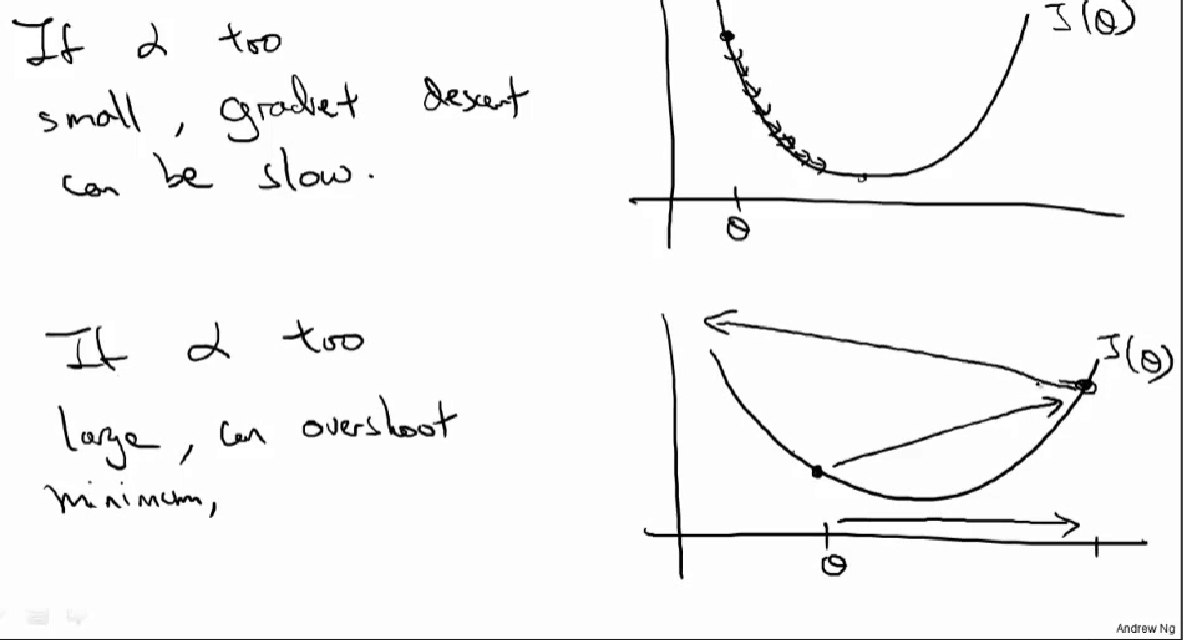
\includegraphics[width=2.5in]{gdeta.png}




\subsection{Linear Regression}
直接用线性回归解决分类问题,在条件高斯噪声分布的假设下,线性模型的最大化似然函数等价于最小化平方和误差函数,可以直接给出参数的解析解。
\par 考虑L2正则化项(和书上的公式不同,我们不把偏置项包括进去):
\[E(\omega)=\frac{1}{2}\sum_{n=1}^{N}(t_n-{\omega}^T\phi(x_n))^2 + \frac{\lambda}{2}\sum_{j=1}^{M}{\omega_j}^2\]
\[\nabla E(\omega)=\sum_{n=1}^{N}(t_n-{\omega}^T\phi(x_n))\phi(x_n)^T + \lambda[0,\omega_1,\omega_2,,,\omega_M]^T\]
\par 令梯度为0:
\[\omega=(\lambda I^{*} +\Phi^T \Phi)^{-1} \Phi^T t\]
\par $I^{*}$除了第一行第一列的元素为0,其他位置和M+1阶单位阵相同。
\par 由此就完成线性回归的参数估计,在分类时,$\omega^T\phi(x)> 0.5$则分为垃圾邮件。
\par 实际上,虽然实验结果还不错,但个人认为线性回归不是分类的理想解决方式,下图显示了一维特征样本上用线性回归做分类的理想(来自cs273a):\\
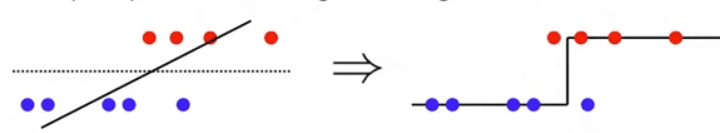
\includegraphics[height=0.6in]{lingood.png}
\\与可能的残酷现实\\
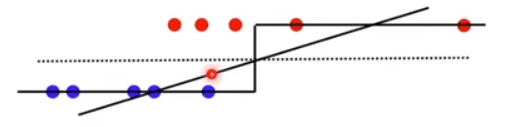
\includegraphics[height=0.6in]{linbad.png}
\paragraph{i}
\par 不同正则化参数下的错误率:\\
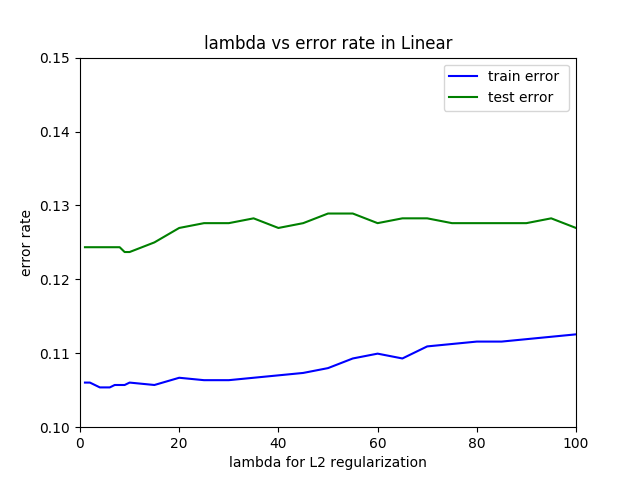
\includegraphics[height=3.8in]{Linear-lam.png}
\paragraph{ii}整体上随着$\lambda$增大,训练集和测试集上的错误率都略有增大,原因和Logistic回归类似不在赘述。
\paragraph{iii}不同预处理下的错误率,二值化和Log操作有比较好的效果。(很难微观上分析原因,只能宏观上说数据这样处理后可能比较符合之前给出的线性回归做分类的理想情况。)
\begin{table}[!htbp]
% \resizebox{1.4\linewidth}{!}
  \centering
  \scalebox{1}{
\begin{tabular}{ l | c | c | c }
  \hline      
  train-err|test-err & $\lambda=1$ & $\lambda=10$ & $\lambda=100$  \\ \hline
  None  & 10.6|12.4 & 10.6|12.3 &11.2|12.6   \\ \hline
  Binarized  & 7.3|7.8 & 7.4|7.9 &7.9|8.5   \\ \hline 
  Z-normalized  & 10.6|11.9 & 10.6|12.1 &11.0|12.8   \\ \hline
  Log  & 6.1|6.5 & 6.0|6.5 &5.9|6.5   \\ \hline 
\end{tabular}
}
\caption{不同预处理下错误率LinearRegression}
\label{tb:lda_knn}
\end{table}

\paragraph{iv}$\lambda$取1,10,100时的错误率已在上题给出。
\paragraph{v}虽然线性回归模型中参数的最大似然估计能直接给出解析解,但是对于大规模数据集,求$(\lambda I^{*} +\Phi^T \Phi)$的逆的操作会比较困难,此时就可以考虑随机梯度下降这样的顺序学习的算法,即:
\[\omega_{r+1}=\omega_r-\eta\nabla En \]
\par 在L2正则化的线性回归模型中:
\[\omega_{r+1}=\omega_r-\eta((\omega_r^T \phi_n - t_n)\phi_n + \lambda \omega_r) \]
\par SGD算法非常非常受训练样本顺序的影响,每次的更新方向只取决于当前样本,添加momentum以后可以保留一定之前的更新方向,传说可以增加学习稳定性,让学习更快:
\[v=\gamma v + \eta\nabla En  \]
\[\omega = \omega - v\]
\par 其中$\gamma$表示之前的更新方向在下一次更新中的权重
\par 本次实验,自己手动实现了SGD+momentum,但即使使用了momentum,在所有参数一致的情况下,仅仅是每次打乱样本顺序重新训练,得到了$13\%$到$71\%$各种不同的错误率,所以为了更加稳定并尽可能让算法收敛,我选择打乱并反复使用训练集500次。
\par 和样本顺序同样重要的,顺序学习的学习率会直接影响算法的收敛,非常不幸的,无预处理+标准的SGD+momentum算法我并没有尝试出最理想的学习率。(各种学习率和其他条件下无预处理错误始终超过$35\%$,而同等条件预处理后错误率大致为:binaried$13\%$,z-norm$13\%$,log$9\%$)
\par 应对无预处理的情况,我增加了学习率“step decay”的策略后得到了相对较好的结果,即每次更新$\omega$后,降低学习率$\eta = \eta *0.5$,如下面两图所示,在训练集顺序使用1次(此时就没有多次使用的意义),$\lambda = 1 (L2), preprocessing = none,\gamma = 0.5,\eta$取$10^{-9}$到$10^{-5}$时,采用普通sgd+momentum和加上学习率下降策略后不同的分类表现。\\
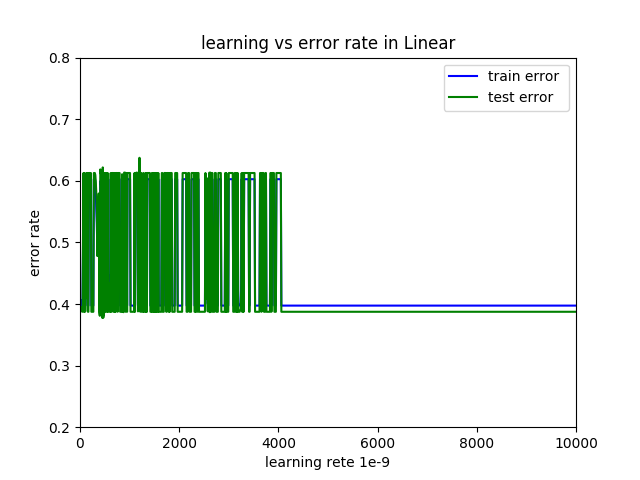
\includegraphics[height=2.3in]{Learningrate1.png}
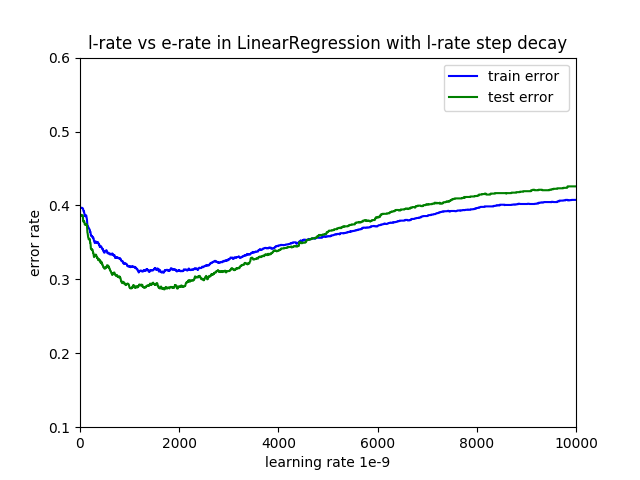
\includegraphics[height=2.3in]{Learningrate2.png}
\par 可以发现,加上学习率下降策略,$\eta$取$[1*10^{-6},2*10^{-6}]$的SGD+momentum相对比较好的。(对于几种预处理后的数据,标准SGD+momentum效果很好,学习率下降策略反而画蛇添足)
\par 由此可以正式回答第5题,做两组实验。实验一、不预处理,$\lambda = 1 (L2),\gamma = 0.5(mom)$,在\ $[10^{-8},5*10^{-6}]$内均匀取500个学习率,顺序使用样本一次,SGD+momentum+学习率下降算法和直接得出最小平方解的算法进行召回率和精确率上的比较。实验二、取对数,$\lambda = 1,\gamma = 0.5$,在$\eta = [1,5,10,,,100]*10^{-5}$,乱序使用样本500次,SGD+momentum算法和直接得出最小平方解的算法进行召回率和精确率上的比较。
\par 本实验中,精确率=正确分出的垃圾邮件/判为垃圾邮件的好坏邮件总数(如果没有分出垃圾邮件人为设成1),召回率=正确分出的垃圾邮件/垃圾邮件总数。
\par 最小平方解无关学习率,仅以直线表示。
\par 实验一,无预处理。\\
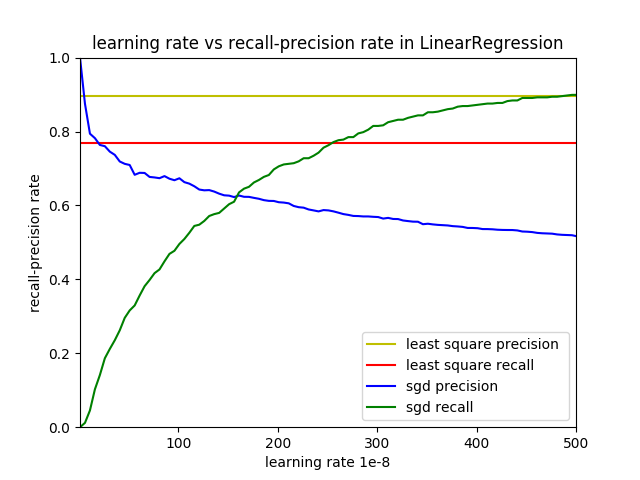
\includegraphics[height=3.8in]{rec-pre.png}
\par 实验二,log预处理。\\
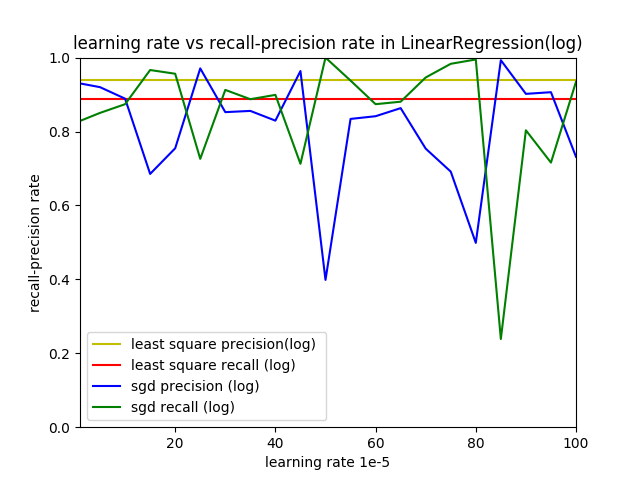
\includegraphics[height=3.7in]{rec-pre3.png}
\par 在$\eta$取$10^{-5}$至$10^{-3}$,乱序使用样本500次后基本SGD能收敛,性能几乎接近了解析解,但是样本顺序不同的影响还是明显超过了学习率的影响,使得分类效果波动特别大。



\subsection{KNN}
\par KNN的模型比较简单,就是对一个新的测试样本,取特征空间上距离最近的几个训练样本,其中哪个类的样本多就分为哪类。KNN的效果除了取决于找几个邻居(K的取值),还取决于如何定义距离。
\paragraph{i}K取值的影响\\
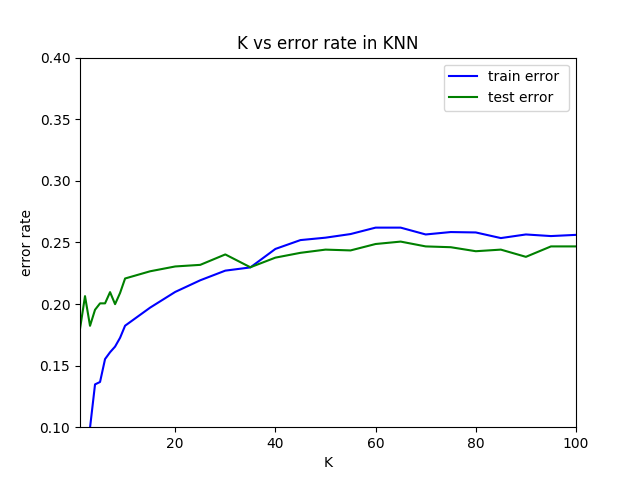
\includegraphics[height=3.8in]{KNN.png}\\
\paragraph{ii} 整体上K增大,错误率提高。在测试集上的表现来讲,KNN取10以内有相对比较好的结果,但有一些波动,当K过大,显然会包括过多与自己特征并不那么接近的点,影响根据近邻判断的效果。
\par K=1在训练集上找KNN,理论上找到自己,不会出错,但实际分错了1份(图上难以表现),原因是本次测试样本中,100号和1333号样本,各特征完全一致,但标签相反,令1333号样本找到最近邻100号样本后分错。
\paragraph{iii}不同预处理下错误率\\
\begin{table}[!htbp]
% \resizebox{1.4\linewidth}{!}
  \centering
  \scalebox{1}{
\begin{tabular}{ l | c | c | c }
  \hline      
  train-err|test-err & $K=1$ & $K=10$ & $K=100$  \\ \hline
  None  & 0.0|17.9 & 18.2|22.0.3 &25.6|24.6   \\ \hline
  Binarized  & 1.1|8.2 & 7.5|8.2 &11.7|11.5   \\ \hline 
  Z-normalized  & 0.0|9.7 & 8.2|10.0 &12.4|13.9   \\ \hline
  Log  & 0.0|6.5 & 5.2|7.0 &8.9|10.5   \\ \hline 
\end{tabular}
}
\caption{不同预处理下错误率KNN}
\label{tb:lda_knn}
\end{table}
\par 由于实验样本提取的特征有几种不同类型,取值差异可以很大,有的集中在比较小的值域,有的值域范围大,方差也大。未经预处理直接计算欧氏距离找KNN可能出现,两个点的许多特征都很近似,但某几个值域范围大的特征上有差异,欧氏距离就很大的情况,实际上以上三种预处理都很大程度上缓解了这一问题。
\par 二值化后多出了一个小问题,就是二值化后出现更多特征完全一致,但不同类的点,所以K=1时在训练集上的错误较高。


\paragraph{iv}上题给出

\section*{survey}
\par 由于进行了系统的复习,看了一些网课,耗时略长,用了4个整天,每天在7-8小时,共计超过30小时。


\bibliographystyle{plain}
\bibliography{report}


\end{document}